\documentclass[12pt,a4paper]{article}

\usepackage[utf8]{inputenc}
\usepackage[a4paper,total={150mm,240mm}]{geometry}
\usepackage[american]{babel}

\usepackage{float}
\usepackage{babel}
\usepackage{amsmath}
\usepackage{tikz}
\usepackage{graphicx}
\usepackage{amssymb}
\usepackage{todonotes}


\usepackage{listings}
\definecolor{listingbg}{gray}{0.95}
\lstset{language=C++,basicstyle=\ttfamily\small,frame=single,backgroundcolor=\color{listingbg}}
% \lstset{language=C++, basicstyle=\ttfamily,
%   keywordstyle=\color{black}\bfseries, tabsize=4, stringstyle=\ttfamily,
%   commentstyle=\it, extendedchars=true, escapeinside={/*@}{@*/}}


\newcommand{\vx}{\vec x}
\newcommand{\grad}{\vec \nabla}
\newcommand{\wind}{\vec \beta}
\newcommand{\Laplace}{\Delta}
\newcommand{\mycomment}[1]{}


% Exercise stylesheet
\usepackage{exercise}

\title{\textbf{Exercises for Tutorial01}}
\subtitle{Poisson with Nonlinearity}
\exerciselabel{Exercise}




\begin{document}

\exerciseheader

The code of tutorial 01 solves the problem
\begin{align*}
  -\Delta u + q(u) &= f &&\text{in $\Omega$},\\
  u &= g &&\text{on $\Gamma_D\subseteq\partial\Omega$},\\
  -\nabla u\cdot \nu &= j &&\text{on $\Gamma_N=\partial\Omega\setminus\Gamma_D$}
\end{align*}
with the nonlinear function $q(u)=\eta u^2$.  It is written in such
a way that dimension, degree of the discretization or the
nonlinearity can easily be changed.

In this exercise you will get to know the code, play around with
different settings and implement a different way to handle the
Dirichlet boundary condition.


\begin{Exercise}{Warming Up}
  First we want to get familiar with the code.
  \begin{enumerate}
  \item Try out different dimensions, grids, polynomial degrees and
    values for $\eta$.  All these settings can be modified through the
    ini file \lstinline{tutorial01.ini} and can be tested without
    rebuilding your program.  Here are some suggestions that could be
    interesting:
    \begin{itemize}
    \item Use higher values for $\eta$.
    \item Go to 3 dimensions and use the contour filter in parview to
      visualize your results.  Hint: Add a range.
    \end{itemize}
    %\begin{figure}[h]
      \begin{center}
        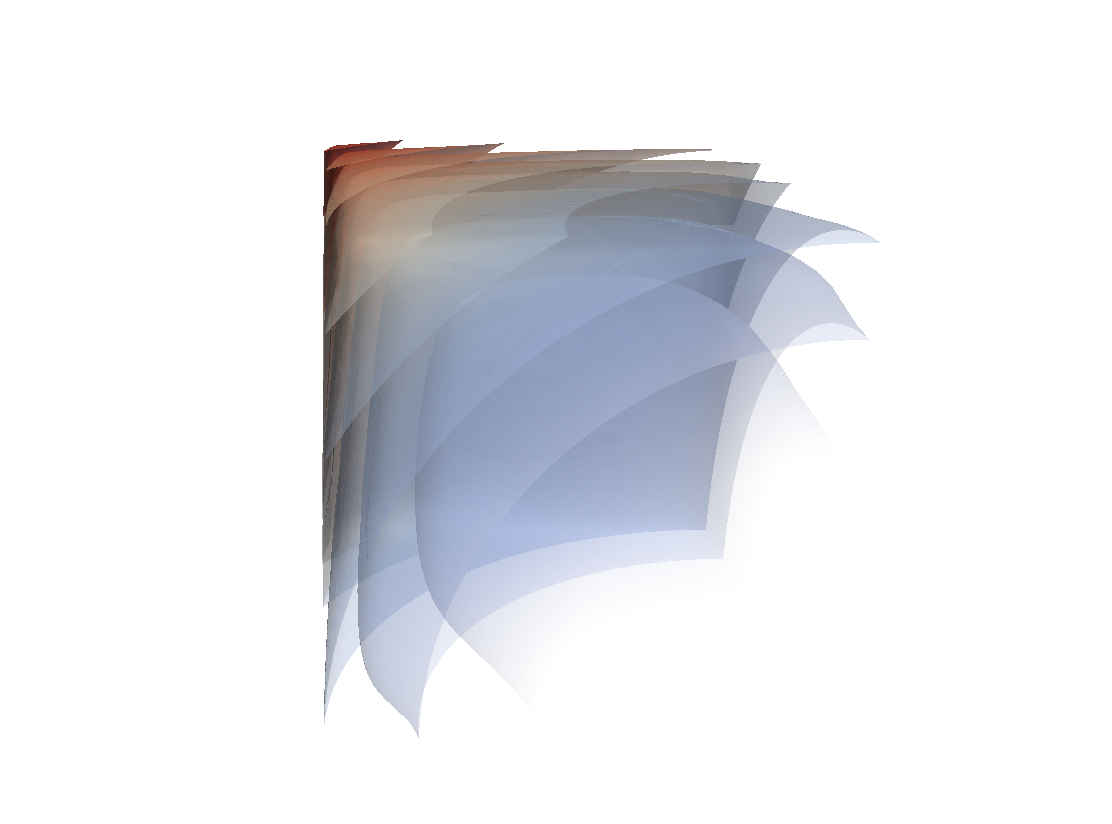
\includegraphics[width=0.9\textwidth]{nonlinear_poisson_contour.png}
      \end{center}
      % \caption{Contour plot of numerical solution in three dimensions
      %   and $\eta=100$.}
    %\end{figure}

  \item Run the code with the following setting:
    \begin{lstlisting}
[grid]
dim=2        # set to 1 | 2 | 3
manager=yasp # set to ug | alu | yasp
refinement=1 # be careful

...

[fem]
degree=1 # oned: 1..4, ug|alu: 1..3, yasp: 1..2

[problem]
eta=2.0

[output]
filename=degree1_subsampling0
subsampling=0
\end{lstlisting}
    Try all combinations of \lstinline{degree=1|2} and
    \lstinline{subsampling=1|2} with appropriate
    \lstinline{filename}.  Look at your solutions using paraview and the
    \lstinline{warp by scalar} filter.  You can see the underlying grid
    by choosing \lstinline{surface with edges} instead of
    \lstinline{surface} in the parview drop down menu.  How does
    subsampling change the output?

  \item It is easy to implement different nonlinearities.  Use
    $q(u)=\exp(au)$ by adjusting the file \lstinline{problem.hh}.

  \item Go back to $q(u)=\eta u^2$.  Now we want to see how good our
    approximation is.  Change the function $f(x)$ in the file
    \lstinline{problem.hh} to $f(x)=-2d+\eta(\sum_{i=1}^d(x)_i^2)^2$
    where $d$ is the dimension (and therefore size of $x$).  Then
    $u(x)=\sum_{i=1}^d(x)_i^2=g(x)$ is the exact solution.  Visualize the
    exact solution like it is done it tutorial 00. We start with the
    ini file
    \begin{lstlisting}
[grid]
dim=2        # set to 1 | 2 | 3
manager=yasp # set to ug | alu | yasp
refinement=1 # be careful

...

[fem]
degree=1 # oned: 1..4, ug|alu: 1..3, yasp: 1..2

[problem]
eta=100.0

[output]
filename=yasp_ref_0
subsampling=0
    \end{lstlisting}
    Use paraview to see how the maximal error $\max|u-u_h|$ behaves
    for diferent refienements \lstinline{refinement=1|...|5}.  Then
    try again for \lstinline{degree=2}.  What happens here?  Does the
    behaviour change when you use \lstinline{alu} instead of
    \lstinline{yasp}?
  \end{enumerate}
\end{Exercise}

\begin{Exercise}{Nitsche's method for weak Dirichlet boundary
    conditions}
  In this exercise we want to implement Dirichlet boundary conditions
  in a weak sense by using Nitsche's method.  Instead of
  incorporating the Dirichlet bounday condition into the Ansatzspace
  we modify the residual:
  \begin{align*}
    r^{\text{Nitsche}}(u,v) &= \int_\Omega \nabla u \cdot \nabla v + (q(u)-f)v\,dx + \int_{\Gamma_N} jv\,ds \\
    &\quad - \int_{\Gamma_D} \nabla u \cdot\nu v\,ds - \int_{\Gamma_D} (u-g)\nabla v \cdot\nu\,ds
    + \eta_{stab} \int_{\Gamma_D} (u-g)v\,ds.
  \end{align*}
  Here $\eta_{stab}$ denotes a stabilization parameter that should be
  equal to $\eta_{stab}=c/h$ for a constant $c>0$ large enough.  This
  stabilization term is needed to ensure coercivity of the bilinear
  form.

  In order to implement this method you have to do the following:
  \begin{itemize}
  \item Go to \lstinline{exercise01.cc} and include the new file
    \lstinline{nitschenonlinearpoissonfem} instead of
    \lstinline{nonlinearpoissonfem}.
  \item In the file \lstinline{driver.hh} you have to turn of the
    constraints.  The code is already ther you just have to
    comment/uncomment the parts marked with
    \begin{lstlisting}
//== Exercise 2 {
...
// ...
//== }
    \end{lstlisting}
    to
    \begin{lstlisting}
//== Exercise 2 {
// ...
...
//== }
    \end{lstlisting}
    By changing these lines you use no constraints, an empty
    constraints container and construct the grid operator without
    constraints.  Besides that you use the new
    \lstinline{NitscheNonlinearPoissonFEM} local operator that expects
    the stabilization parameter $\eta_{stab}$.
  \item The key part is adding the \lstinline{alpha_boundary} method
    to the new local operator in the file
    \lstinline{nitschenonlinearpoissonfem.hh}.  Take a close look at
    the \lstinline{lambda_volume}, \lstinline{lambda_boundary} and
    \lstinline{alhpa_volume} methods and you should be on your way.

    \emph{Hint:} The code for generating the transformation
    is already there:
    \begin{lstlisting}
// transform gradients of shape functions to real element
const auto S = geo_inside.jacobianInverseTransposed(local);
    \end{lstlisting}

  \end{itemize}

  When you have done all that test your implementation.  Use the test
  case from exercise 1 with $f(x)=-2d+\eta(\sum_{i=1}^d(x)_i^2)^2$ and
  exact solution $u(x)=\sum_{i=1}^d(x)_i^2=g(x)$ and compare it to
  your approximation.

  Introduce the parameter
  \begin{lstlisting}
[fem]
stab = 100
  \end{lstlisting}
  in the ini file and look at the maximal error $\max|u-u_h|$ for
  \lstinline{stab=10|100|1000.}
\end{Exercise}


\end{document}
